%!TEX root = ../thesis.tex
% ******************************* Thesis Appendix E ********************************

\chapter{Alignment of the Setup}
\label{appendix:align}

The configuration of the telescope was measured manually in the laboratory. For an ideal setup, sensor layers are aligned precisely along the beam axis, with positions of the form (0,0,z). However, manual assembly could introduce misalignments, particularly in the transverse (x,y) directions and rotations about the z axis. Displacements on the order of of $10^{-4}$m are common, which are comparable to the pixel pitch of the sensor and could lead to incorrect or failed fits. If the misalignment reaches $10^{-3}$m, track constructions may no longer be feasible. Therefore, the setup must be aligned by software before analysis can proceed. 

The alignment procedure in Corryvreckan involves three steps, beginning with prealignment, which gives an initial estimate of the misalignment - typically on the order of $10^{-3}$m to $10^{-4}$m. This is done by calculating the spatial correlations, $x_{correlation}$ and $y_{correlation}$, where
\begin{equation}
    x_{correlation} = x_{detector} - x_{reference}
    \label{eq:correlation}
\end{equation}
refers to the local spatial difference\footnote{Note that the spatial correlations can be calculated without track information, so tracking is not required for prealignments.} between clusters on the reference detector and those on target detectors. This is performed with the \texttt{Correlations} module. In an ideal setup, the peak of the correlation distribution would be centred around zero; in practice, there are typically offsets due to misalignment. However, for large initial offsets, an effective initial guess is to shift detector positions to align the correlation peak with zero. Then, with a relatively loose matching criteria, track reconstruction becomes possible.


Next, the \texttt{AlignmentTrackChi2} module is used to perform automated and more precise alignment. Non-reference telescope planes are shifted along x,y directions and rotated about the z axis, and tracks are refitted with the trial geometries to minimise $\chi^2$ values using Minuit2\cite{Minuit}. This process is performed iteratively until the alignment converges to a stable configuration. The resulting geometry is written into an output file for subsequent analysis. However, it is possible that the angular orientations does not converge, due to the rotational symmetry of the setup and the telescope plane about z axis. 

\begin{figure}[h!] 
\centering    
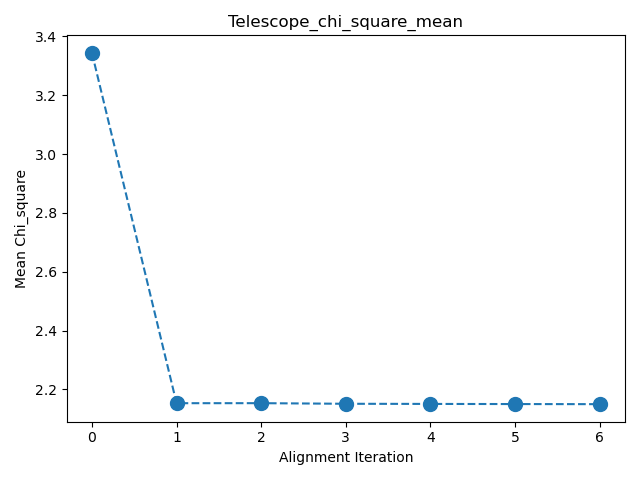
\includegraphics[width=0.6\linewidth]{4_Methods/Figs/TrackChi.png}
\caption{The change of mean $\chi^2$ value of the tracks during telescope alignment.}
\end{figure}


The result of the alignment is checked with the x,y residuals calculated by the \texttt{AnalysisTelescope} module, where
\begin{equation}
    x_{residual} = x_{cluster} - x_{track}
    \label{eq:correlation}
\end{equation}
refers to the difference between the position of the associated cluster and the track intersection on telescope planes. Unlike correlations, residuals are track-dependent. The goal of a fine-tuned alignment is to minimise spatial residuals and centre their distributions at zero\footnote{In contrast, spatial correlation peaks may remain offset due to the inherent differences between the x,y position of detector planes.}.

A similar procedure can be applied to the DUT by the \texttt{AlignmentDUTResidual} module, where only the DUT position is modified.

\begin{figure}[h!] 
\centering    
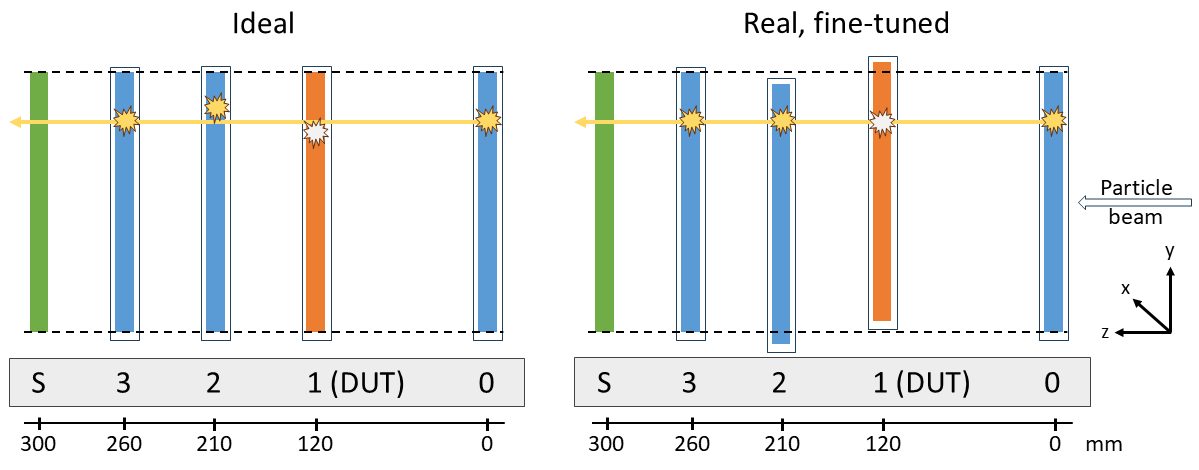
\includegraphics[width=.9\linewidth]{4_Methods/Figs/Alignment.png}
\caption{An illustration of a straight track fit through an (left) ideal and (right) fine-tuned, real alignment. Offsets are exaggerated for clarity. In the fine-tuned case, spatial residuals are centred around zero, indicating good alignment, while spatial correlations are offset due to difference in detector positioning.}
\label{img:Alignment}
\end{figure}